



\documentclass{article}\usepackage{graphicx, color}
%% maxwidth is the original width if it is less than linewidth
%% otherwise use linewidth (to make sure the graphics do not exceed the margin)
\makeatletter
\def\maxwidth{ %
  \ifdim\Gin@nat@width>\linewidth
    \linewidth
  \else
    \Gin@nat@width
  \fi
}
\makeatother

\IfFileExists{upquote.sty}{\usepackage{upquote}}{}
\definecolor{fgcolor}{rgb}{0.2, 0.2, 0.2}
\newcommand{\hlnumber}[1]{\textcolor[rgb]{0,0,0}{#1}}%
\newcommand{\hlfunctioncall}[1]{\textcolor[rgb]{0.501960784313725,0,0.329411764705882}{\textbf{#1}}}%
\newcommand{\hlstring}[1]{\textcolor[rgb]{0.6,0.6,1}{#1}}%
\newcommand{\hlkeyword}[1]{\textcolor[rgb]{0,0,0}{\textbf{#1}}}%
\newcommand{\hlargument}[1]{\textcolor[rgb]{0.690196078431373,0.250980392156863,0.0196078431372549}{#1}}%
\newcommand{\hlcomment}[1]{\textcolor[rgb]{0.180392156862745,0.6,0.341176470588235}{#1}}%
\newcommand{\hlroxygencomment}[1]{\textcolor[rgb]{0.43921568627451,0.47843137254902,0.701960784313725}{#1}}%
\newcommand{\hlformalargs}[1]{\textcolor[rgb]{0.690196078431373,0.250980392156863,0.0196078431372549}{#1}}%
\newcommand{\hleqformalargs}[1]{\textcolor[rgb]{0.690196078431373,0.250980392156863,0.0196078431372549}{#1}}%
\newcommand{\hlassignement}[1]{\textcolor[rgb]{0,0,0}{\textbf{#1}}}%
\newcommand{\hlpackage}[1]{\textcolor[rgb]{0.588235294117647,0.709803921568627,0.145098039215686}{#1}}%
\newcommand{\hlslot}[1]{\textit{#1}}%
\newcommand{\hlsymbol}[1]{\textcolor[rgb]{0,0,0}{#1}}%
\newcommand{\hlprompt}[1]{\textcolor[rgb]{0.2,0.2,0.2}{#1}}%

\usepackage{framed}
\makeatletter
\newenvironment{kframe}{%
 \def\at@end@of@kframe{}%
 \ifinner\ifhmode%
  \def\at@end@of@kframe{\end{minipage}}%
  \begin{minipage}{\columnwidth}%
 \fi\fi%
 \def\FrameCommand##1{\hskip\@totalleftmargin \hskip-\fboxsep
 \colorbox{shadecolor}{##1}\hskip-\fboxsep
     % There is no \\@totalrightmargin, so:
     \hskip-\linewidth \hskip-\@totalleftmargin \hskip\columnwidth}%
 \MakeFramed {\advance\hsize-\width
   \@totalleftmargin\z@ \linewidth\hsize
   \@setminipage}}%
 {\par\unskip\endMakeFramed%
 \at@end@of@kframe}
\makeatother

\definecolor{shadecolor}{rgb}{.97, .97, .97}
\definecolor{messagecolor}{rgb}{0, 0, 0}
\definecolor{warningcolor}{rgb}{1, 0, 1}
\definecolor{errorcolor}{rgb}{1, 0, 0}
\newenvironment{knitrout}{}{} % an empty environment to be redefined in TeX

\usepackage{alltt}
\usepackage[margin=1.5in]{geometry}
\usepackage{algorithm, color, algpseudocode, amsmath, url, geometry, ctable }
\usepackage[square,numbers]{natbib}
\setlength{\marginparwidth}{1.2in}
\newcommand{\marginnote}[1]{\-\marginpar[\raggedleft\footnotesize #1]{\raggedright\footnotesize #1}}
\newcommand{\todo}[1]{\marginnote{\textcolor{red}{TODO #1}}}
\newcommand{\mc}[1]{\todo{(MC) #1}}

%{\marginpar{ \textcolor{red}{\\ TODO: #1 \\} }
\begin{document}

\title{Hippocampal segmentation with MAGeT}
\author{Jon Pipitone}
\maketitle

\begin{abstract}
Neuroimaging research often relies on automated anatomical segmentations of MR
images of the brain. Current multi-atlas based approaches provide accurate
segmentations of brain images by propagating manually derived segmentations of
specific neuroanatomical structures to unlabelled data. These approaches often
rely on a large number of such manually segmented atlases that take significant
time and expertise to produce. We present an algorithm for the automatic
segmentation of the hippocampus that minimizes the number of atlases needed
while still achieving similar accuracy to multi-atlas approaches.
\todo{Finish this... }
\end{abstract}

\section{Introduction}

The hippocampus is of particular interest to many researchers because it is
implicated in forms of brain dysfunction such as Alzheimer's disease and
schizophrenia, and has functional significance in cognitive processes such as
learning and memory.  For many research questions involving magnetic resonance
imaging (MRI) data accurate identification of the hippocampus and its
subregions is a necessary first step to better understand the individual
neuroanatomy of subjects.  

Currently, the gold standard for neuroanatomical segmentation is manual
delineation by an expert human rater.  This is problematic for segmentation of
the hippocampus for several reasons.  First, manual segmentation takes a
significant investment of time and expertise \citep{Hammers2003} which may not
be readily available to researchers or clinicians.  Second, the amount of data
produced in neuroimaging experiments increasingly exceeds the capacity for
identification of specific neuroanatomical structures by an expert manual
rater.  Third, the true definition of hippocampal anatomy in MR images is
disputed \citep{Geuze2004}, as evidenced by efforts to create an unified
segmentation protocol \citep{Jack2011}.  

Compounding each of these problems is the significant neuroanatomical
variability in the hippocampus throughout the course of aging, development, and
neuropsychiatric disorders \citep{Mouiha2011}.  Additionally, it may be
necessary to use several different hippocampal definitions or, in fact, make
specific modifications in the course of research. For example, Poppenk et al.
\citep{Poppenk2011} found that subdividing the hippocampus into anterior and
posterior regions resulted in a predictive relationship between volume
difference of those regions and recollection memory performance.  Thus, while
manual segmentation of the hippocampus is a necessary technique, to researchers
or clinicians who do not have access to the needed human expertise its use may
be infeasible.  

Automated segmentation techniques overcome the need for human expertise by
performing segmentations computationally.  A popular class of automated
methods, {\it multi-atlas-based segmentation}, rely on a set of expertly
labeled neuroanatomical atlases. Each atlas is warped to fit a subject's
neuroanatomy using nonlinear registration
techniques \citep{Collins1995,Klein2009}.  Atlas labels are then transformed by
this warping and a {\it label fusion} technique, such as voxel-wise voting, is
used to merge the competing label definitions from each atlas into a final
segmentation for a subject.  

Many descriptions of multi-atlas-based segmentation algorithms report relying
on an atlas library containing anywhere between 30 and 80 expertly labeled
brains \citep{Heckemann2011,Collins2010,Aljabar2009,Leung2010,Lotjonen2010}.  As
noted, the production of an atlas library requires significant manual effort,
and is limited since the choice of atlases or segmentation protocol may not
reflect the underlying neuroanatomical variability of the population under
study or be suited to answer the research questions at hand.

In this paper we propose an automated segmentation method to address the above
issues of existing multi-atlas-based methods. Principally, our method aims to
dramatically reduce the number of manually labelled atlases needed (under 10).
This is achieved by using the small atlas library to boot-strap a much larger
"template library", which is then used to segment the subjects in a similar
fashion to basic multi-atlas segmentation. This approach has the additional
advantage of using the unique subject population on hand to initialize the
segmentation process and improve accuracy.

The essential insight of generating a template library is not new.  Heckemann
\citep{Heckemann2006} compared generating a template library from a single atlas
to standard multi-atlas segmentation and found poor performance and so deemed
the approach as inviable.  The LEAP algorithm \citep{Wolz2010} proceeds by
iteratively segmenting the unlabelled image most similar to the atlas library
images and then incorporating the now-labelled image into the atlas library,
but requires 30 starting atlases.  The novelty of our method is to demonstrate
the possibility of producing comparable segmentation accuracy to these and
other multi-atlas-based methods while using significantly fewer manually
created atlases.

In our previous work \citep{Chakravarty2012}, we applied MAGeT brain to
segmentation of the human striatum, globus pallidus, and thalamus using a
single histologically-derived atlas. The main contribution of this paper is to
extend our approach to the human hippocampus and perform a thorough validation
over a range of atlas and template library sizes, which was not done in our
previous work.  Due to the small number of atlases required, our method can
easily accommodate different hippocampal definitions. Our aim is not to improve
on segmentation accuracy beyond existing methods, but instead to provide a
method that trades off manual segmentation expertise for computational
processing time while providing sufficient accuracy for clinical and research
applications.

\section{Materials and Methods}


explain two registration methods, definitions, fusion methods. 
compare to each other, and then compare atlas-based, true multi-atlas, naive methods.
trying to make choices as to the best reg/fusion/

evaluations
described previously in Chakravarty2012. 

\subsection{Segmentation Algorithm}
\todo{Make sure we explain what MAGeT stands for}
In this paper, we use the term {\it atlas} to mean any manually segmented MR
image, and the term {\it atlas library} to mean a set of such images.  We use
the term {\it template} to refer to any MR image, and associated labelling,
used to segment another image, and the term {\it template library} to refer to
a set of such images.  An atlas library may be used as a template library but,
as we will discuss, a template library may also be composed of images with
computer generated labellings. 

The segmentation approach we propose is best understood as an extension of
basic multi-atlas segmentation \citep{Collins2010}.  In multi-atlas segmentation,
an atlas library and unlabelled MR images are given as input.  Every atlas
image is nonlinearly registered to each unlabelled image, and then each atlas'
labels are propagated via the resulting transformations.  These labels are then
fused to produce a single, definitive segmentation by some label fusion method
(e.g.  voxel-wise majority vote). 

Our extension adds a preliminary stage in which a template library is
constructed from input images, and used in place of an atlas library in the
standard multi-atlas-based method.  To create the template library, labels from
each atlas image are propagated to each template library image via the
transformation resulting from a non-linear registration between pair of images.
As a result, each template library image has a label from each atlas.
Basic multi-atlas segmentation is then used to produce segmentations for the
entire set of unlabelled images (including those images used in the template
library). 

Label fusion is performed by cross-correlation weighted voting, a strategy
weighted towards an optimal combination of subjects from the template library
which has been previously shown to improve segmentation
accuracy \citep{Aljabar2009,Collins2010}. In this method, each template library
image is ranked in similarity to each unlabelled image by the normalized
cross-correlation of image intensities after linear registration in a region of
interest (ROI) generously encompassing the hippocampus.  Only the top ranked
template library image labels are used in a voxel-wise majority vote. The ROI
is heuristically defined as the extent of all atlas labels after linear
registration to the template, dilated by three voxels \citep{Chakravarty2012}.

Source code can be found at \url{http://github.com/pipitone/MAGeTbrain}.

\begin{algorithm}
\caption{Pseudocode for the MAGeT Brain algorithm}
\label{pseudocodesdf}
\begin{algorithmic}
\Function{MultiAtlas}{Templates, Subjects}
  \ForAll{$subject$}
    \ForAll{$template$}
      \State propagate all labels for template to subject space
      \State store subject labels
    \EndFor
    \State fuse subject labels
  \EndFor
\EndFunction
\\
\Function {MAGeTBrain}{Subjects, Atlases, n}
  \For{$i = 1 \to n$}
    \State choose a subject to be used as a template
    \State propagate labels from each atlas to template space
    \State store the template with all of its labels
  \EndFor
  \State MultiAtlas(Templates, Subjects)
\EndFunction
\end{algorithmic}
\end{algorithm}

\begin{figure}[h]
  \centering
    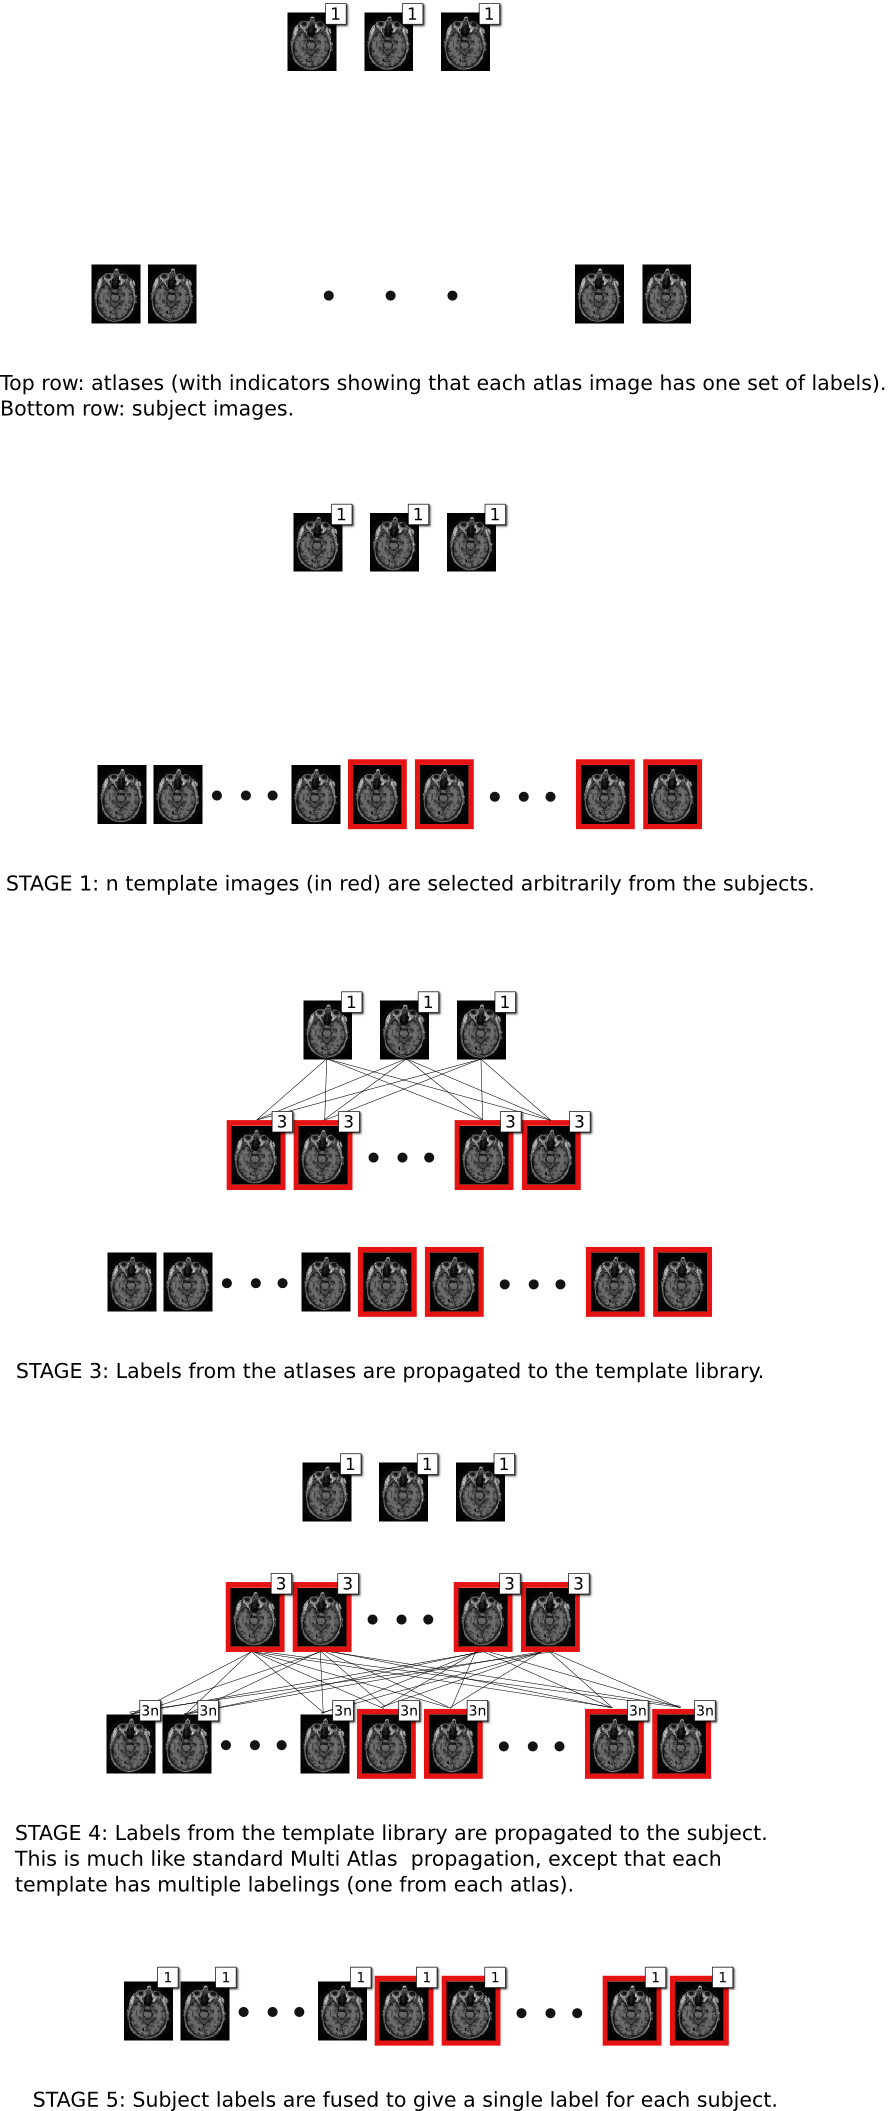
\includegraphics[width=0.5\textwidth]{figure/MAGeT-figure.png}
  \caption{Diagram of the MAGeT Brain algorithm}
\end{figure}

\subsection{Image Processing and Registration Methods}

Before images were registered, the N3 algorithm [16] is first used to minimize
the intensity nonuniformity in each of the atlases and unlabeled subject
images. In this work we investigated the performance of two registration
methods.  

\subsubsection{Automatic Normalization and Image Matching and Anatomical Labeling (ANIMAL)}

The ANIMAL algorithm carries out Image registration is in two phases. In the
first, a 12-parameter linear transformation (3 translations, rotations, scales,
shears) is estimated between images using an algorithm that maximizes the
correlation between blurred MR intensities and gradient magnitude over the
whole brain \citep{Collins}. In the second phase, nonlinear registration is completed using
the ANIMAL algorithm \citep{Collins1995}: an iterative procedure that estimates a 3D
deformation field between two MR images. At first, large deformations are
estimated using blurred version of the input data. These larger deformations
are then input to subsequent steps where the fit is refined by estimating
smaller deformations on data blurred with a Gaussian kernel with a smaller
FWHM. The final transformation is a set of local translations defined on a bed
of equally spaced nodes that were estimated through the optimization of the
correlation coefficient. 

For the purposes of this work we used the
regularization parameters optimized in Robbins et al. \citep{Robbins2004}. It
should be noted that the MAGeT brain algorithm is not dependent on this, or
any, particular choice of registration method \citep{Chakravarty2012}.

\todo{should add the MNI website here; also we should add the parameters we used somewhere}

\subsubsection{Automatic Normalization Tools (ANTS)}

ANTs is a diffeomorphic registration algorithm which provides great flexibility
over the choice of transformation model, objective function, and the
consistency of the final transformation. The transformation is estimated in a
hierarchical fashion where the MRI data is subsampled, allowing large
deformations to be estimated and successively refined at later hierarchical
stages (where the data is subsampled to a finer grid). The deformation field
and the objective function are regularized with a Gaussian kernel at each level
of the hierarchy. The ANTs algorithm is freely available
\url{http://www.picsl.upenn.edu/ANTS/}. We used an implementation of the ANTS
algorithm compatible with the MINC data format, mincANTS
\url{https://github.com/vfonov/mincANTS} \todo{(same here we should add the
parameters we used).}

\subsection{Label Fusion Methods}

Label fusion is term given to the process of combining the information from
several candidate labellings for an MR image into a single labelling.  In this
paper we explore the benefits of three different fusion methods. 

\subsubsection{Voxel-wise Majority Vote}

Labels are propagated from all template library images to a subject.  Each
output voxel is given the most frequent label at that voxel location amongst
all candidate labellings.  Ties are broken arbitrarily.

\subsubsection{Cross-correlation Weighted Majority Vote}

Labels are propagated from only those template library images which most
similar to the subject.  A voxel-wise majority vote is carried out from the
labels from the top n ranked template library images, where n is parameter set
by the user. 

Similarity between a subject and a template image is measured using normalized
cross-correlation of intensity values, over a region of interest defined on
each template, after the subject has been linearly registered to the template.
The heuristic used for defining a meaningful region of interest for each
template is to use the extent of all the propagated labellings from each atlas
(after linear registration only) and then dilating this region by three voxels.
 
The utility to calculate the cross-correlation similarity measure is
implemented as part of the ANIMAL toolkit. \todo{(ANIMAL or MINC)}

\subsubsection{Normalised Mutual Information Weighted Majority Vote}

This label fusion method is identical to the above process except a normalised
mutual information score is used over the region of interest between a template
and subject instead of cross-correlation.  

The utility to calculate the normalised mutual information measure is
implemented as part of the EZMinc package (based on ITK NMI routine).

\subsection{Goodness-of-fit}

Each segmentation was evaluated against the 'gold-standard' manual segmentation
from the dataset using the Dice Kappa ($\kappa$) overlap metric:

\begin{equation*} 
\kappa=\frac{2a}{2a+b+c}
\end{equation*}

where $a$ is the number of voxels common to the candidate segmentation and the
gold standard and $b+c$ is the sum of the voxels uniquely identified by either
the automatically generated candidate segmentation or the gold-standard.
\todo{I would do this after you define the experiments}

\subsection{Data and Experiments}

Three different experiments were conducted to evaluate the influence of
registration method, atlas set size and resolution, template set size, and
label fusion method and parameters.


%%%%%%%%%%%%%%%%%%%%%%%%%%%%%%%%%%%%%%%%%%%%%%%%%%%%%%%%%%%%%%%%%%%%%%%%%%%%%%%
%                         Experiment Rationale 
%%%%%%%%%%%%%%%%%%%%%%%%%%%%%%%%%%%%%%%%%%%%%%%%%%%%%%%%%%%%%%%%%%%%%%%%%%%%%%%
\definecolor{shadecolor}{rgb}{0.969, 0.969, 0.969}\color{fgcolor}\begin{kframe}
\subsubsection{Study Method Rationale - An Outline}
\begin{description}
\item[ADNI Repeated Random Subsampling Validation] \hfill \\ 
{\bf Purpose:} to validate robustness of MAGeT accuracy when atlas set is representative 
of subject set w.r.t. registration method, atlas and template library composition and size, and 
various fusion methods. Additionally, to choose the best configuration of parameters 
(under the assumption that performance generalises). 
\\ \\ 
{\bf Method:} using a set of 69 ADNI subjects, 13 from each disease category, perform 
10 rounds of repeated random subsampling to pick atlas library and template library 
for each parameter setting and then run MAGeT brain to segment non-atlas subjects.
Also perform multi-atlas and single-atlas segmentation using the same parameter settings
and atlas library size.
\\ \\
{\bf Results:} find significant improvement over multi-atlas performed with the same
parameters. Also, find smoothed performance is monotonically increasing but asymptotic
in size of both template and atlas library, with peak performance reached after 15
templates. \todo{Can we statistically capture "peak" performance?  The point at which 
gains become statistically insignificant?}

\item[Winterburn Atlas Reliability] \hfill \\
{\bf Purpose:} validation of reliability of whole hippocampus and hippocampal 
subregion segmentations.
\\ \\
{\bf Method:} we use the Winterburn atlas set, using each high-res atlas in turn 
to segment a standard-res MR of the same subject and compare the automatic 
segmentation to the atlas segmentation.  We use a template library consisting 
of standard-res MRs from the remaining Winterburn atlas subjects plus 11 other 
standard-res healthy control subjects. 
\\ \\
{\bf Results:} TBD 

\item[Winterburn-Atlas ADNI Baseline Segmentation] \hfill \\
{\bf Purpose:} given that MAGeT is robust and accurate, show MAGeT performance on a real-world task in which atlas set may not be representative of subjects.
\\ \\
{\bf Method:} We use best settings from first experiment (ANTS, majority vote, 
template library of 20), and use Winterburn hi-res atlases to segment all ADNI Baseline 
images.  Since our segmentation protocol differs from what can be segmented at 
ADNI resolution a direct comparison is not appropriate.  Instead, we validate by 
showing how well our segmentation volumes correlate with existing automated/manual 
segmentation volumes. \todo{Also show disease prediction?}
\\ \\
{\bf Results: } 

\item[First Episode SZ Patients Segmentation] \hfill \\ 
{\bf Purpose:} validate MAGeT's general performance.
\\ \\
{\bf Method:} Measure performance on a different disease dataset. We use FEP SZ patients and controls, 
using two different atlas sets: a manual hippocampal segmentation of patients, and Winterburn 
atlas set.  We validate the native-atlas set segmentations using Dice's Kappa, 
and the Winterburn-atlas-set segmentations by correlating volumes. 
\\ \\
{\bf Results:} High volume correlation between Winterburn segmentation volumes and ground truth.  (High-ish?) Kappa when using manual segmentations as Atlases. 

\end{description}
\end{kframe}

\subsubsection{ADNI Validation Experiment}

In this experiment we performed repeated random sub-sampling cross-validation
of the MAGeT algorithm with a pool of 69 images and labels from the ADNI
dataset.  The images are T1-weighted \todo{<insert description of scan/machine
types>}.  The hippocampal labels are provided as part of the ADNI dataset, and
are produced \todo{<insert description of SNT labellings>}.  The parameters we
varied, and the ranges over which we varied are listed in \todo{table}.  We
performed 10 validations per parameter combination.  In each validation trial,
a random sample of subjects were chosen from the pool without replacement as
the atlas set, whereas the template set was chosen randomly with replacement.   

\begin{table}
    \begin{tabular}{l|l}
        Parameter           & Values tested                                                      \\ \hline
        Number of Templates & 3 to 20                                                            \\ 
        Number of Atlases   & 3 to 9                                                             \\ 
        Registration Method & ANTS or ANIMAL                                                     \\ 
        Label Fusion Method & majority vote, cross-correlation weighted vote, NMI weighted vote. 
    \end{tabular}
\end{table}

We used the following parameters for ANTS, during registration: 
\begin{verbatim}
  mincANTS 3 -m PR[target_file.mnc,source_file.mnc,1,4] 
   --number-of-affine-iterations 10000x10000x10000x10000x10000 
   --affine-gradient-descent-option 0.5x0.95x1.e-4x1.e-4
   --use-Histogram-Matching --MI-option 32x16000
   -r Gauss[3,0] -t SyN[0.5] -i 100x100x100x20
   -o transformation.xfm
 \end{verbatim}
These settings were adapted from the "reasonable starting point" given in the
ANTS manual. \todo{<rationale?>}

For the purposes of this work we used the regularization parameters optimized
in Robbins et al.[15]. \todo{right? (but added a second layer).}

\todo{multi-atlas comparison, "naive" comparison}

\subsubsection{Winterburn High-resolution Hippocampal Atlas - ADNI Validation}

In this experiment we explored using the MAGeT brain algorithm with the
Winterburn high-resolution atlases to segment 21 randomly chosen MR images from
the ADNI dataset (seven each of healthy, MCI and AD subjects).  The Winterburn
atlases are digital segmentations of the hippocampus in five  in-vivo 300u
isotropic T1-weighted MR scans, and include subfield segmentations for the
cornus ammonis (CA) 1, CA4, dentate gyrus, subiculum, and CA 2 and 3 combined.
Subjects in the Winterburn atlases range in age from 29-57 years (mean age of
37), and include two males and three females.  

Since hippocampal segmentation protocols differ between the ADNI labels and
Winterburn atlases, this poses a problem for direct similarity comparisons
between labels produced by MAGeT brain and the ADNI labels.  \todo{explain why
we did(n't) resegment the ADNI images with a the low-res protocol.} To evaluate
the performance of MAGeT brain, we compared classification accuracy of subjects
by diagnosis based on hippocampal volume using both the SMT labels and our
produced labels.  \todo{description of validation -- rms {\tt validate} or
t-test: contrast with QDA or LDA (Coupe 2011) used in LOOCV}


% latex.default(cstats, title = title, caption = caption, rowlabel = rowlabel,      col.just = col.just, numeric.dollar = FALSE, insert.bottom = legend,      rowname = lab, dcolumn = dcolumn, extracolheads = extracolheads,      extracolsize = Nsize, ...) 
%
{\scriptsize\ctable[caption={Descriptive Statistics by Baseline Dx},label=tab,rotate]{lccccc}{\tnote[]{\noindent {\scriptsize $a$\ }{$b$\ }{\scriptsize $c$\ } represent the lower quartile $a$, the median $b$, and the upper quartile $c$\ for continuous variables.}\tnote[]{Numbers after percents are frequencies.}\tnote[]{\indent Tests used:}\tnote[]{\textsuperscript{\normalfont 1}Kruskal-Wallis test; \textsuperscript{\normalfont 2}Pearson test}}{\FL
\multicolumn{1}{l}{}&\multicolumn{1}{c}{CN}&\multicolumn{1}{c}{LMCI}&\multicolumn{1}{c}{AD}&\multicolumn{1}{c}{Combined}&\multicolumn{1}{c}{Test Statistic}\NN
&\multicolumn{1}{c}{{\scriptsize $N=23$}}&\multicolumn{1}{c}{{\scriptsize $N=23$}}&\multicolumn{1}{c}{{\scriptsize $N=23$}}&\multicolumn{1}{c}{{\scriptsize $N=69$}}&\ML
Age~at~baseline~\hfill\tiny{Years}&{\scriptsize 72.2~}{75.5 }{\scriptsize 78.5} &{\scriptsize 71.0~}{77.1 }{\scriptsize 81.4} &{\scriptsize 71.7~}{77.8 }{\scriptsize 81.8} &{\scriptsize 71.5~}{76.6 }{\scriptsize 81.3} &$ F_{2,66}=0.15 ,~ P=0.862 ^{1} $\NN
Sex~:~Female&43\%~{\scriptsize~(10)}&43\%~{\scriptsize~(10)}&43\%~{\scriptsize~(10)}&43\%~{\scriptsize~(30)}&$ \chi^{2}_{2}=0 ,~ P=1 ^{2} $\NN
Education&{\scriptsize 16.0~}{16.0 }{\scriptsize 18.0} &{\scriptsize 15.0~}{16.0 }{\scriptsize 18.0} &{\scriptsize 12.0~}{16.0 }{\scriptsize 16.5} &{\scriptsize 14.0~}{16.0 }{\scriptsize 18.0} &$ F_{2,66}=3.44 ,~ P=0.038 ^{1} $\NN
Marital~status~at~baseline~:~Married&74\%~{\scriptsize~(17)}&87\%~{\scriptsize~(20)}&87\%~{\scriptsize~(20)}&83\%~{\scriptsize~(57)}&$ \chi^{2}_{4}=3.04 ,~ P=0.551 ^{2} $\NN
~~~~Widowed&22\%~{\scriptsize~(~5)}&13\%~{\scriptsize~(~3)}&13\%~{\scriptsize~(~3)}&16\%~{\scriptsize~(11)}&\NN
~~~~Divorced&~4\%~{\scriptsize~(~1)}&~0\%~{\scriptsize~(~0)}&~0\%~{\scriptsize~(~0)}&~1\%~{\scriptsize~(~1)}&\NN
~~~~Never~married&~0\%~{\scriptsize~(~0)}&~0\%~{\scriptsize~(~0)}&~0\%~{\scriptsize~(~0)}&~0\%~{\scriptsize~(~0)}&\NN
~~~~Unknown&~0\%~{\scriptsize~(~0)}&~0\%~{\scriptsize~(~0)}&~0\%~{\scriptsize~(~0)}&~0\%~{\scriptsize~(~0)}&\NN
Ethnicity~:~Unknown&~~0\%~{\scriptsize~(~0)}&~~0\%~{\scriptsize~(~0)}&~~0\%~{\scriptsize~(~0)}&~~0\%~{\scriptsize~(~0)}&$^{2}$\NN
~~~~Not~Hisp/Latino&100\%~{\scriptsize~(23)}&100\%~{\scriptsize~(23)}&100\%~{\scriptsize~(23)}&100\%~{\scriptsize~(69)}&\NN
~~~~Hisp/Latino&~~0\%~{\scriptsize~(~0)}&~~0\%~{\scriptsize~(~0)}&~~0\%~{\scriptsize~(~0)}&~~0\%~{\scriptsize~(~0)}&\NN
Race~:~Am~Indian/Alaskan&~~0\%~{\scriptsize~(~0)}&~~0\%~{\scriptsize~(~0)}&~~0\%~{\scriptsize~(~0)}&~~0\%~{\scriptsize~(~0)}&$ \chi^{2}_{2}=5.61 ,~ P=0.061 ^{2} $\NN
~~~~Asian&~~0\%~{\scriptsize~(~0)}&~~0\%~{\scriptsize~(~0)}&~~0\%~{\scriptsize~(~0)}&~~0\%~{\scriptsize~(~0)}&\NN
~~~~Hawaiian/Other~PI&~~0\%~{\scriptsize~(~0)}&~~0\%~{\scriptsize~(~0)}&~~0\%~{\scriptsize~(~0)}&~~0\%~{\scriptsize~(~0)}&\NN
~~~~Black&~17\%~{\scriptsize~(~4)}&~~4\%~{\scriptsize~(~1)}&~~0\%~{\scriptsize~(~0)}&~~7\%~{\scriptsize~(~5)}&\NN
~~~~White&~83\%~{\scriptsize~(19)}&~96\%~{\scriptsize~(22)}&100\%~{\scriptsize~(23)}&~93\%~{\scriptsize~(64)}&\NN
~~~~More~than~one&~~0\%~{\scriptsize~(~0)}&~~0\%~{\scriptsize~(~0)}&~~0\%~{\scriptsize~(~0)}&~~0\%~{\scriptsize~(~0)}&\NN
~~~~Unknown&~~0\%~{\scriptsize~(~0)}&~~0\%~{\scriptsize~(~0)}&~~0\%~{\scriptsize~(~0)}&~~0\%~{\scriptsize~(~0)}&\NN
CDR-SB&{\scriptsize 0.00~}{0.00 }{\scriptsize 0.00} &{\scriptsize 0.75~}{1.50 }{\scriptsize 1.50} &{\scriptsize 4.00~}{4.50 }{\scriptsize 5.00} &{\scriptsize 0.00~}{1.50 }{\scriptsize 4.00} &$ F_{2,66}=294 ,~ P<0.001 ^{1} $\NN
ADAS~13&{\scriptsize  4.67~}{ 5.67 }{\scriptsize 12.34} &{\scriptsize 14.34~}{16.00 }{\scriptsize 20.50} &{\scriptsize 23.83~}{29.00 }{\scriptsize 31.66} &{\scriptsize 10.00~}{16.00 }{\scriptsize 25.33} &$ F_{2,66}=110 ,~ P<0.001 ^{1} $\NN
MMSE&{\scriptsize 28.5~}{29.0 }{\scriptsize 30.0} &{\scriptsize 25.0~}{27.0 }{\scriptsize 28.0} &{\scriptsize 21.0~}{23.0 }{\scriptsize 24.0} &{\scriptsize 24.0~}{27.0 }{\scriptsize 29.0} &$ F_{2,66}=94.2 ,~ P<0.001 ^{1} $\LL
}}




\todo{For minctracc -- we registered to TAL}

\subsection{Results}
\subsubsection{A2A}

Kappa vs. Number of templates: 
Smoothing line fitted using GAM (generalised additive model) from R with defaults from ggplot2 (formula: y ~ s(x, bs = "cs"))
\begin{knitrout}
\definecolor{shadecolor}{rgb}{0.969, 0.969, 0.969}\color{fgcolor}

{\centering 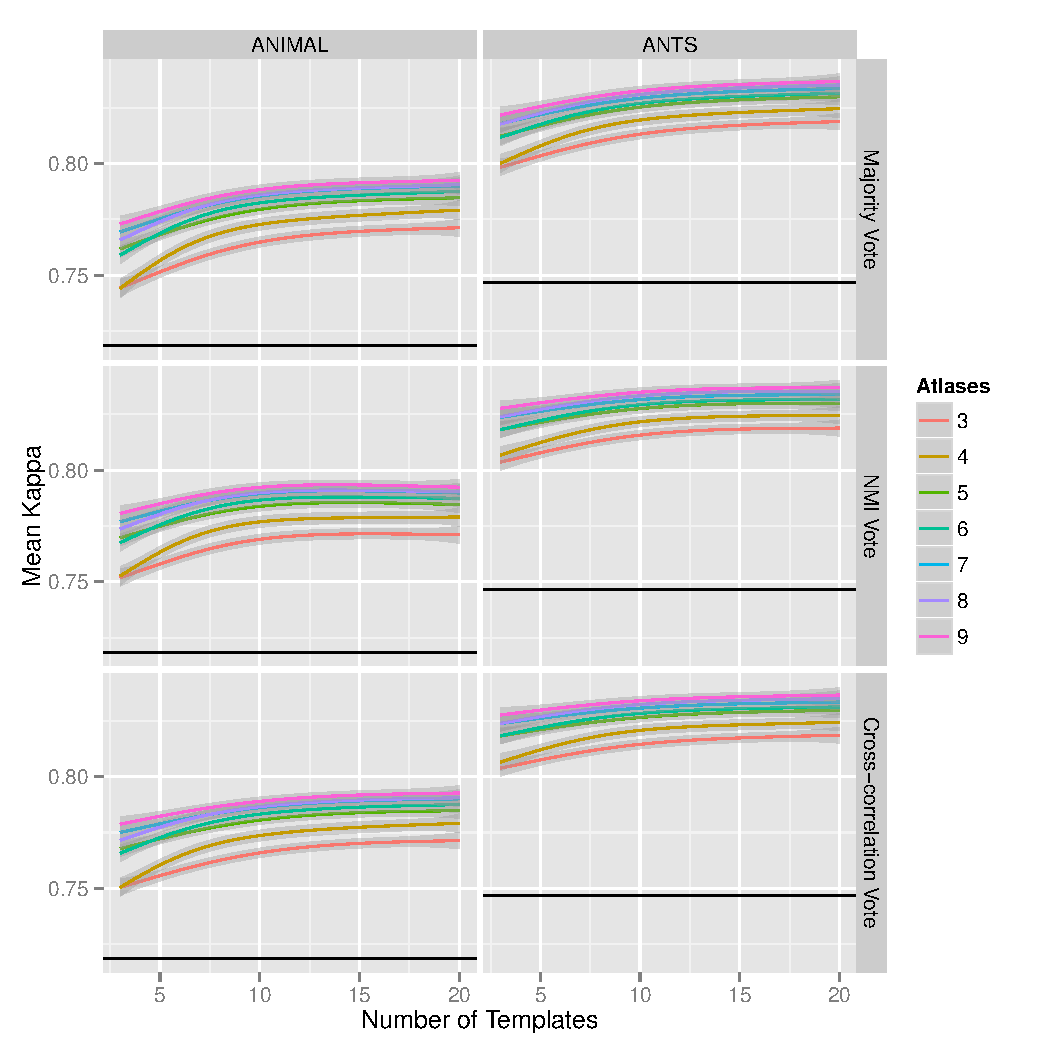
\includegraphics[width=\maxwidth]{figure/a2a_facet} 

}


\end{knitrout}


\begin{knitrout}
\definecolor{shadecolor}{rgb}{0.969, 0.969, 0.969}\color{fgcolor}

{\centering 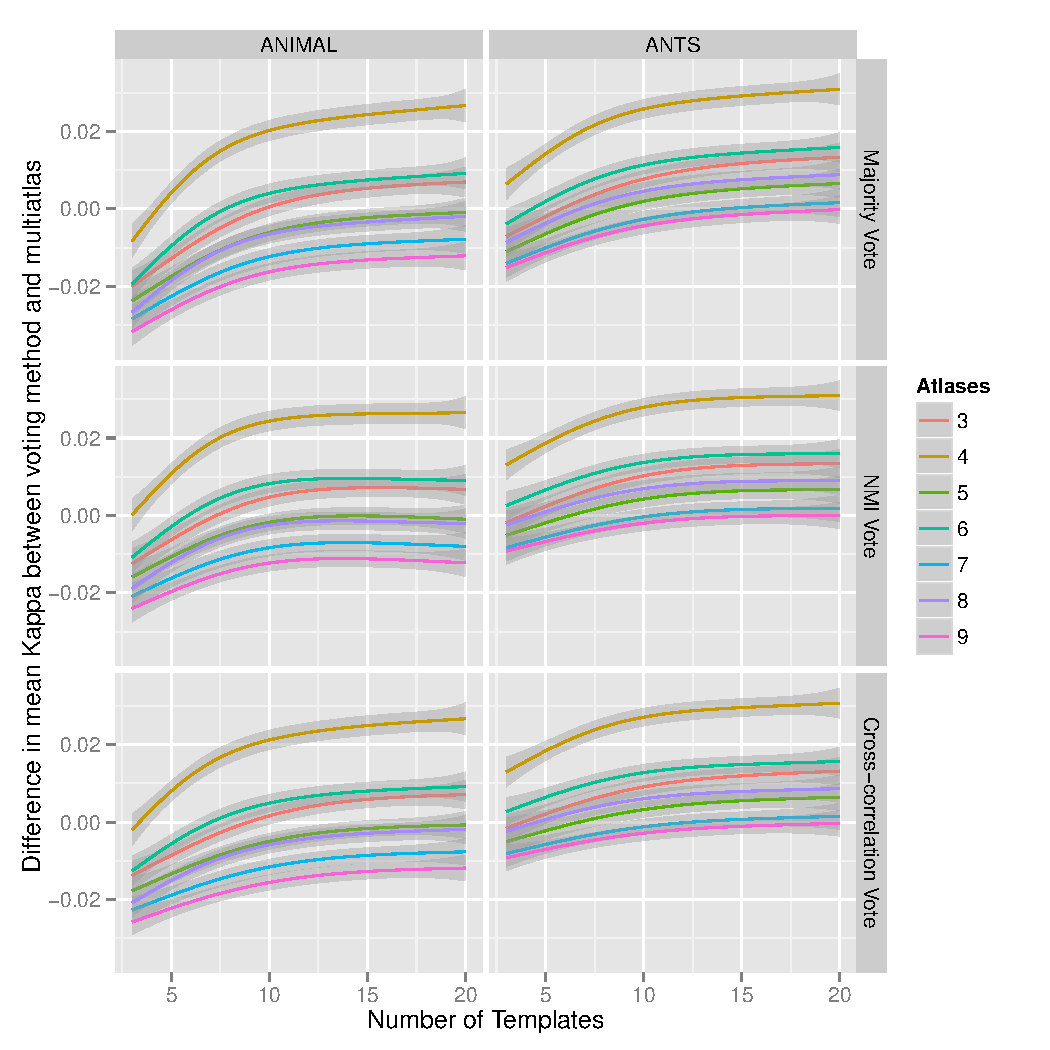
\includegraphics[width=\maxwidth]{figure/a2a_facet_mameans} 

}


\end{knitrout}



Kappa minus multi-atlas mean vs. Number of Templates

Multi-atlas means:


% latex.default(merge(a_ma_means, t_ma_means, by = "num_atlases"),      colheads = c("Atlases", "ANTS", "ANIMAL"), file = "") 
%
\begin{table}[!tbp]
\begin{center}
\begin{tabular}{lrrr}
\hline\hline
\multicolumn{1}{l}{merge}&\multicolumn{1}{c}{Atlases}&\multicolumn{1}{c}{ANTS}&\multicolumn{1}{c}{ANIMAL}\tabularnewline
\hline
1&$3$&$0.805414417498623$&$0.764266832660852$\tabularnewline
2&$4$&$0.793646605043623$&$0.752420649183594$\tabularnewline
3&$5$&$0.823292141139203$&$0.785546924392891$\tabularnewline
4&$6$&$0.815578947302174$&$0.778345910844141$\tabularnewline
5&$7$&$0.831936342756014$&$0.797761650124922$\tabularnewline
6&$8$&$0.826298462726884$&$0.792443538092187$\tabularnewline
7&$9$&$0.836877632304638$&$0.804568318173359$\tabularnewline
\hline
\end{tabular}
\end{center}
\end{table}




\begin{table}
    \begin{tabular}{c|c|c}
        Number of Atlases & ANIMAL Kappa (Jaccard) & ANTS Kappa (Jaccard) \\ \hline
        3                 & 0.76 (0.63)             & 0.80 (0.69)          \\ 
        4                 & 0.75 (0.62)             & 0.79 (0.67)          \\ 
        5                 & 0.79 (0.66)             & 0.82 (0.71)          \\ 
        6                 & 0.78 (0.65)             & 0.82 (0.70)          \\ 
        7                 & 0.80 (0.67)             & 0.83 (0.72)          \\ 
        8                 & 0.79 (0.67)             & 0.83 (0.72)          \\ 
        9                 & 0.80 (0.68)             & 0.84 (0.73)          \\
    \end{tabular}
\end{table}

- more atlases -> better performance
- larger template library -> better performance, but tails off around 10-15 templates
- no significant difference between majority or weighted vote methods (haven???t tested this statistically though). 
- consistently performs better than average naive performance by XXX
- using ANTS, with a large enough template library (>12) MAGeT brain performs
  better than the average multi-atlas approach with the same number of atlases.
  using ANIMAL, 5 or more atlases needed before boost seen. 
- more atlases -> smaller template library required to improve on average multi-atlas performance
- discuss variance?  best/worst case? --how often do we expect random template library selection to work decently

\todo{cost (in registrations) / benefit trade off graph:  show number of registrations per Kappa?  or hours of manual labour per Kappa?)}

\subsubsection{Winterburn Atlas Segmentation of ADNI Baseline Images}

- A2A shows that if atlas population strongly(?) represents subject set
  variability, then free choice from atlas population will produce improvements
(we know this b/c of extensive validation trials). 
- what about in the case where atlas population doesn???t strongly represent
  subject set variability (e.g. a priori atlas set)?  then, we can use atlas
selection to refine atlas set? 

\todo{Kappa against our manual rater is low}




\begin{figure}[h]
\begin{knitrout}
\definecolor{shadecolor}{rgb}{0.969, 0.969, 0.969}\color{fgcolor}

{\centering 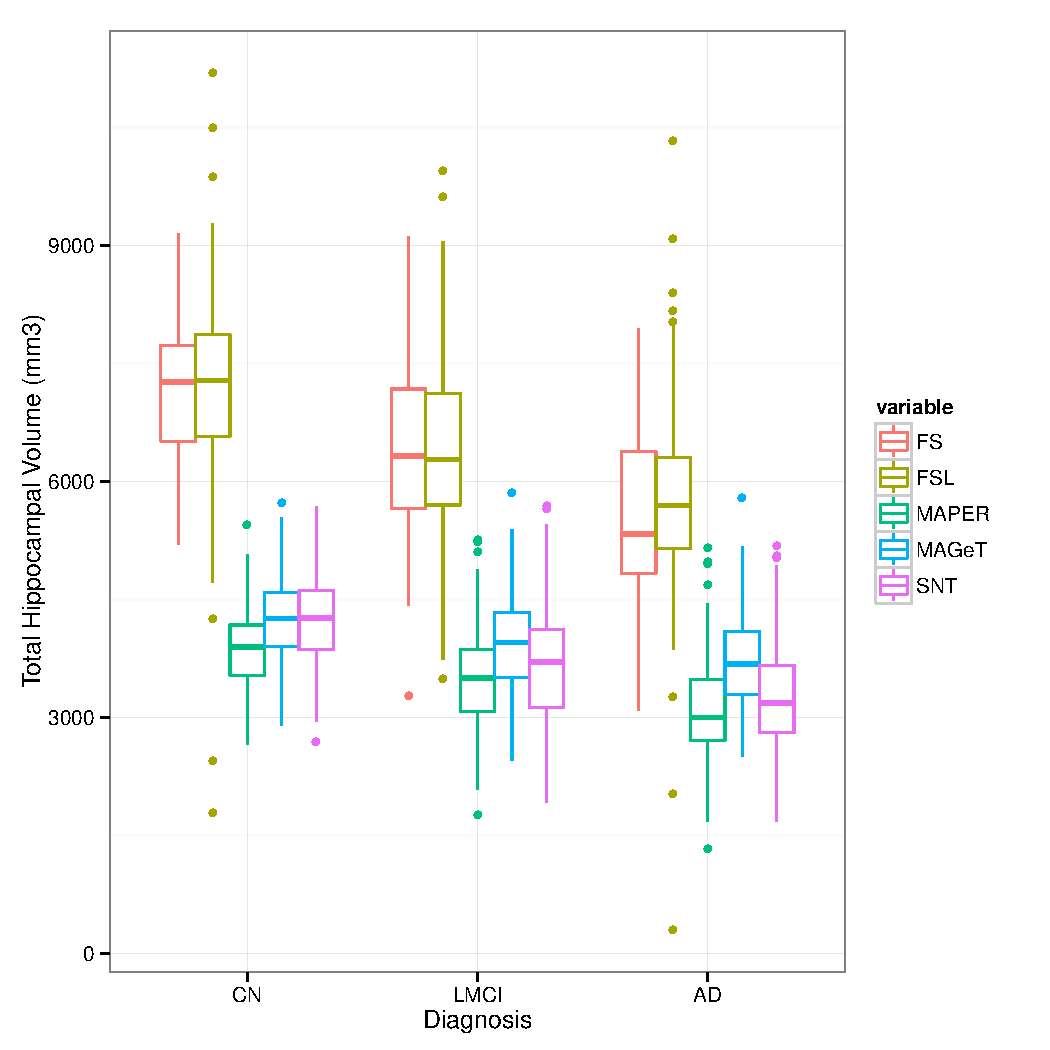
\includegraphics[width=\maxwidth]{figure/ADNI-baseline-volumes-boxplot} 

}


\end{knitrout}

  \caption{Comparison of HC volumes by FreeSurfer (FSF), MAGeT brain (MAGeT), MAPER, and manual (SNT).}
  \label{ADNI-baseline-volumes-boxplot}
\end{figure}

\begin{figure}[h]
\begin{knitrout}
\definecolor{shadecolor}{rgb}{0.969, 0.969, 0.969}\color{fgcolor}

{\centering 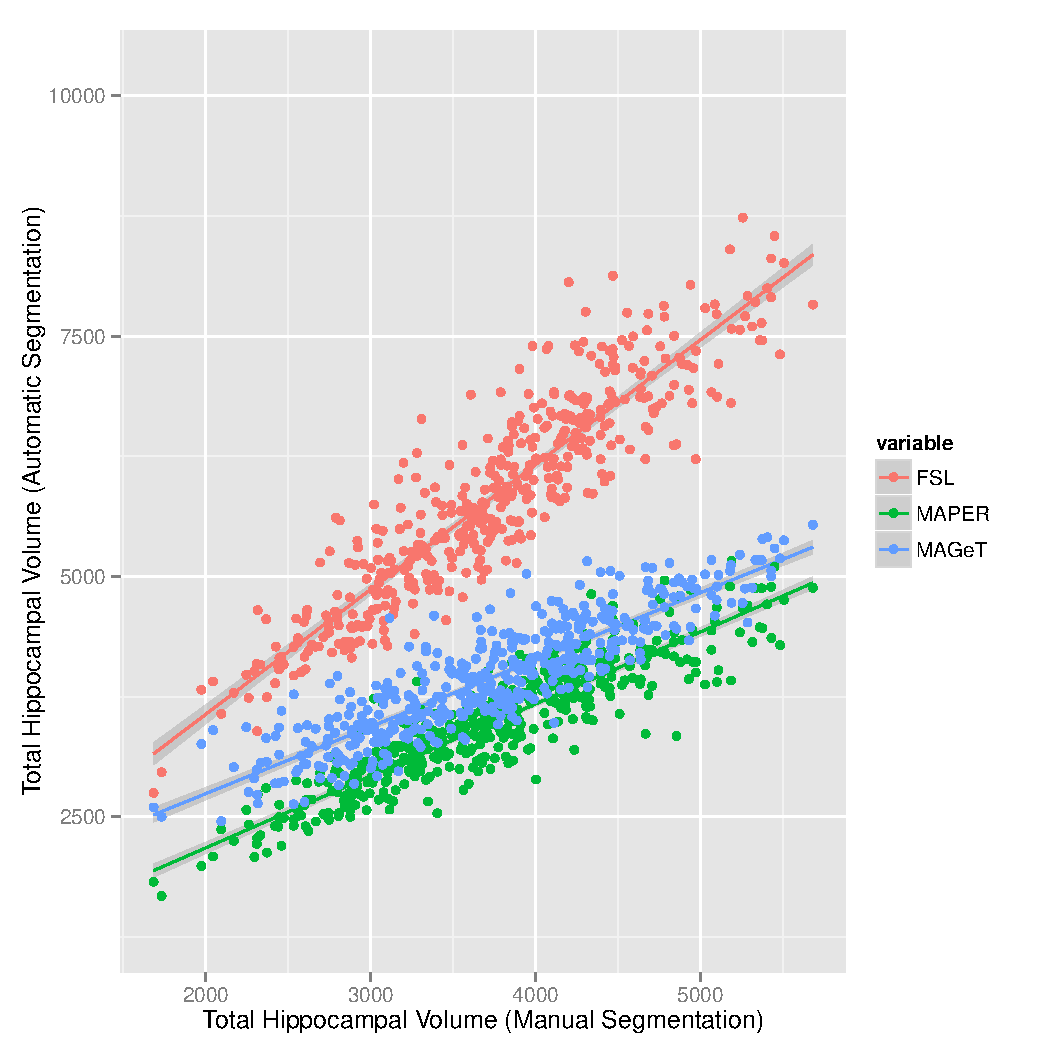
\includegraphics[width=\maxwidth]{figure/ADNI-baseline-volumes-plot} 

}


\end{knitrout}

  \caption{{\bf ADNI Baseline cohort.} Comparison of HC volumes by FreeSurfer (FSF), MAGeT brain (MAGeT), MAPER, and manual (SNT).}
  \label{ADNI-baseline-volumes-plot}
\end{figure}

\subsubsection{First Episode Schizophrenic patients}


% latex.default(cstats, title = title, caption = caption, rowlabel = rowlabel,      col.just = col.just, numeric.dollar = FALSE, insert.bottom = legend,      rowname = lab, dcolumn = dcolumn, extracolheads = extracolheads,      extracolsize = Nsize, ...) 
%
\begin{table}[h]
\scriptsize
\caption{Descriptive Statistics by DX\label{tab}} 
\begin{center}
\begin{tabular}{lrc}
\hline\hline
\multicolumn{1}{l}{}&\multicolumn{1}{c}{N}&\multicolumn{1}{c}{FEP}\tabularnewline
&&\multicolumn{1}{c}{{\scriptsize $N=81$}}\tabularnewline
\hline
Age&80&{\scriptsize 21~}{23 }{\scriptsize 26} \tabularnewline
Gender~:~M&81&63\%~{\scriptsize~(51)}\tabularnewline
Handedness~:~ambi&81&~6\%~{\scriptsize~(~5)}\tabularnewline
~~~~left&&~5\%~{\scriptsize~(~4)}\tabularnewline
~~~~right&&89\%~{\scriptsize~(72)}\tabularnewline
Education&81&{\scriptsize 11~}{13 }{\scriptsize 15} \tabularnewline
SES~:~lower&81&31\%~{\scriptsize~(25)}\tabularnewline
~~~~middle&&54\%~{\scriptsize~(44)}\tabularnewline
~~~~upper&&15\%~{\scriptsize~(12)}\tabularnewline
FSIQ&79&{\scriptsize  88~}{102 }{\scriptsize 109} \tabularnewline
\hline
\end{tabular}
\end{center}
\noindent {\scriptsize $a$\ }{$b$\ }{\scriptsize $c$\ } represent the lower quartile $a$, the median $b$, and the upper quartile $c$\ for continuous variables.\\$N$\ is the number of non--missing values.\\Numbers after percents are frequencies.\end{table}





\begin{figure}
\begin{knitrout}
\definecolor{shadecolor}{rgb}{0.969, 0.969, 0.969}\color{fgcolor}

{\centering 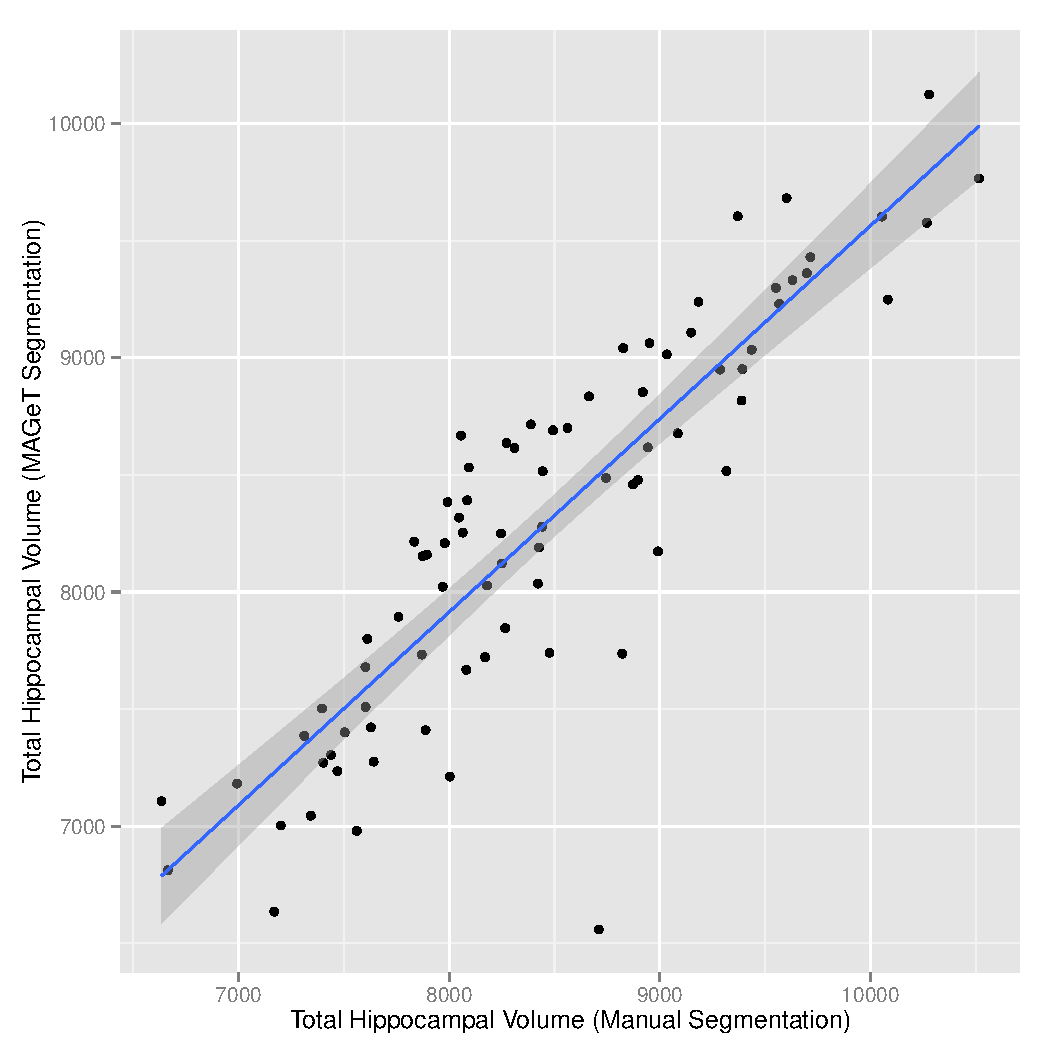
\includegraphics[width=\maxwidth]{figure/SZ_volumes} 

}


\end{knitrout}

  \caption{{\bf First Episode Schizophrenic Patients.} Comparison of total HC volumes for MAGeT against manually rated volumes of}
  \label{SZ_volumes}
\end{figure}

Some other text here... 
\end{document}
